\documentclass[]{article}
\usepackage{lmodern}
\usepackage{amssymb,amsmath}
\usepackage{ifxetex,ifluatex}
\usepackage{fixltx2e} % provides \textsubscript
\ifnum 0\ifxetex 1\fi\ifluatex 1\fi=0 % if pdftex
  \usepackage[T1]{fontenc}
  \usepackage[utf8]{inputenc}
\else % if luatex or xelatex
  \ifxetex
    \usepackage{mathspec}
  \else
    \usepackage{fontspec}
  \fi
  \defaultfontfeatures{Ligatures=TeX,Scale=MatchLowercase}
\fi
% use upquote if available, for straight quotes in verbatim environments
\IfFileExists{upquote.sty}{\usepackage{upquote}}{}
% use microtype if available
\IfFileExists{microtype.sty}{%
\usepackage{microtype}
\UseMicrotypeSet[protrusion]{basicmath} % disable protrusion for tt fonts
}{}
\usepackage[margin=1in]{geometry}
\usepackage{hyperref}
\hypersetup{unicode=true,
            pdftitle={Scientific papers on `Taper functions'},
            pdfauthor={prof. Roberto Scotti},
            pdfborder={0 0 0},
            breaklinks=true}
\urlstyle{same}  % don't use monospace font for urls
\usepackage{natbib}
\bibliographystyle{plainnat}
\usepackage{graphicx,grffile}
\makeatletter
\def\maxwidth{\ifdim\Gin@nat@width>\linewidth\linewidth\else\Gin@nat@width\fi}
\def\maxheight{\ifdim\Gin@nat@height>\textheight\textheight\else\Gin@nat@height\fi}
\makeatother
% Scale images if necessary, so that they will not overflow the page
% margins by default, and it is still possible to overwrite the defaults
% using explicit options in \includegraphics[width, height, ...]{}
\setkeys{Gin}{width=\maxwidth,height=\maxheight,keepaspectratio}
\IfFileExists{parskip.sty}{%
\usepackage{parskip}
}{% else
\setlength{\parindent}{0pt}
\setlength{\parskip}{6pt plus 2pt minus 1pt}
}
\setlength{\emergencystretch}{3em}  % prevent overfull lines
\providecommand{\tightlist}{%
  \setlength{\itemsep}{0pt}\setlength{\parskip}{0pt}}
\setcounter{secnumdepth}{0}
% Redefines (sub)paragraphs to behave more like sections
\ifx\paragraph\undefined\else
\let\oldparagraph\paragraph
\renewcommand{\paragraph}[1]{\oldparagraph{#1}\mbox{}}
\fi
\ifx\subparagraph\undefined\else
\let\oldsubparagraph\subparagraph
\renewcommand{\subparagraph}[1]{\oldsubparagraph{#1}\mbox{}}
\fi

%%% Use protect on footnotes to avoid problems with footnotes in titles
\let\rmarkdownfootnote\footnote%
\def\footnote{\protect\rmarkdownfootnote}

%%% Change title format to be more compact
\usepackage{titling}

% Create subtitle command for use in maketitle
\newcommand{\subtitle}[1]{
  \posttitle{
    \begin{center}\large#1\end{center}
    }
}

\setlength{\droptitle}{-2em}

  \title{Scientific papers on `Taper functions'}
    \pretitle{\vspace{\droptitle}\centering\huge}
  \posttitle{\par}
    \author{prof. Roberto Scotti \footnote{NuoroForestrySchool -
  \href{mailto:scotti@uniss.it}{\nolinkurl{scotti@uniss.it}}}}
    \preauthor{\centering\large\emph}
  \postauthor{\par}
      \predate{\centering\large\emph}
  \postdate{\par}
    \date{21 ago 2018}

\usepackage{array}
\usepackage{fontspec}
\usepackage{hyperref}
\usepackage[labelformat=empty]{caption}

\begin{document}
\maketitle

\hypertarget{introduction}{%
\section{Introduction}\label{introduction}}

\hypertarget{forest-inventory-course---first-results-of-the-collective-assignement}{%
\subsection{2018 Forest Inventory course - First results of the
collective
assignement}\label{forest-inventory-course---first-results-of-the-collective-assignement}}

Students, as homework, were asked to search for scientific papers
presenting `taper functions' and to compile a collective Rmarkdown
document shared using GIT.\\
Rearranging their work, this document lists their findings.

\hypertarget{analysed-articles}{%
\section{Analysed articles}\label{analysed-articles}}

\renewcommand{\arraystretch}{2}

\% Default value: 1

\captionof{table}{
Article ID 1 : _(Scolforo, McTague, Raimundo, et al., 2018)_
**Comparison of taper functions applied to eucalypts of varying genetics in {Brazil}: application and evaluation of the penalized mixed spline approach**
}
\begin{tabular}{p{0.2\textwidth} p{0.8\textwidth}}
\hline
Student & NA \\ \hline
Title.student & Comparison of taper functions applied to eucalypts of varying genetics in Brazil: Application and evaluation of the penalized mixed spline approach \\ \hline
Authors.student & Scolforo, H.F., McTague, J.P., Raimundo, M.R., Weiskittel, A., Carrero, O., Scolforo, J.R.S. \\ \hline
Year.student & 2017 \\ \hline
Species & Eucalypts \\ \hline
Base.URL & http://www.nrcresearchpress.com/doi/10.1139/cjfr-2017-0366#.W2Sb6Lhx02w \\ \hline
Paper.local.file & NA \\ \hline
Equations & NA \\ \hline
\end{tabular}

\captionof{table}{
Article ID 2 : _(Warner, Jamroenprucksa, and Puangchit, 2016)_
**Development and evaluation of teak ({Tectona} grandis {L}.f.) taper equations in northern {Thailand}**
}
\begin{tabular}{p{0.2\textwidth} p{0.8\textwidth}}
\hline
Student & Angelo Manca \\ \hline
Title.student & Development and evaluation of teak (Tectona grandis L.f.) taper equations in northern Thailand, \\ \hline
Authors.student & Andrew J. Warner, Monton Jamroenprucksa, Ladawan Puangchit, \\ \hline
Year.student & 2016 \\ \hline
Species & Tectona grandis L.f. \\ \hline
Base.URL & https://www.sciencedirect.com/science/article/pii/S2452316X16302459?via%3Dihub \\ \hline
Paper.local.file & 1-s2.0-S2452316X16302459-main.pdf \\ \hline
Equations & 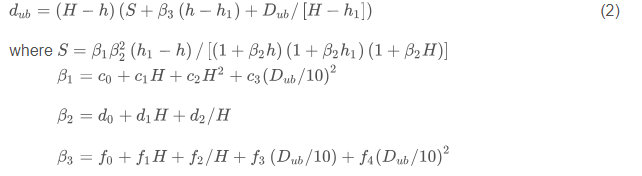
\includegraphics[width=0.8\textwidth]{Equations/2016WarnerEtAl.png} \\ \hline
\end{tabular}

\captionof{table}{
Article ID 3 : _(Tang, Pérez-Cruzado, Fehrmann, et al., 2016)_
**Development of a {Compatible} {Taper} {Function} and {Stand}-{Level} {Merchantable} {Volume} {Model} for {Chinese} {Fir} {Plantations}**
}
\begin{tabular}{p{0.2\textwidth} p{0.8\textwidth}}
\hline
Student & NA \\ \hline
Title.student & Development of a Compatible Taper Function and Stand-Level Merchantable Volume Model for Chinese Fir Plantations \\ \hline
Authors.student & Xiaolu Tang,César Pérez-Cruzado,Lutz Fehrmann,Juan Gabriel Álvarez-González,Yuanchang Lu,and Christoph Kleinn, \\ \hline
Year.student & 2016 \\ \hline
Species & Cunninghamia lanceolata [Lamb.] Hook \\ \hline
Base.URL & https://www.ncbi.nlm.nih.gov/pubmed/26799399 \\ \hline
Paper.local.file & pone.0147610.pdf \\ \hline
Equations & 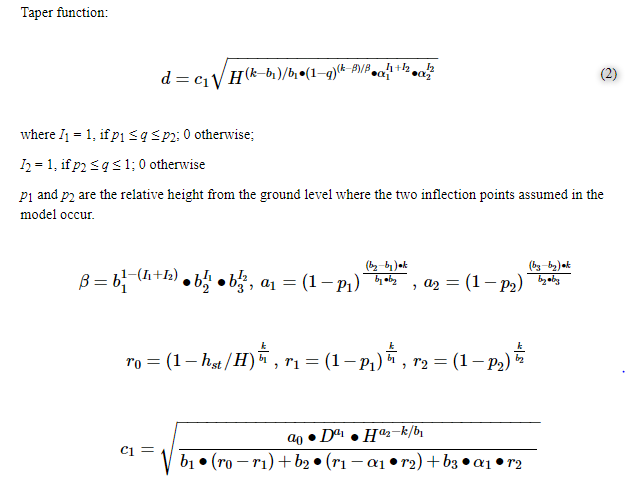
\includegraphics[width=0.8\textwidth]{Equations/2016TangEtAl.png} \\ \hline
\end{tabular}

\captionof{table}{
Article ID 4 : _(Corral-Rivas, Vega-Nieva, Rodríguez-Soalleiro, et al., 2017)_
**Compatible {System} for {Predicting} {Total} and {Merchantable} {Stem} {Volume} over and under {Bark}, {Branch} {Volume} and {Whole}-{Tree} {Volume} of {Pine} {Species}**
}
\begin{tabular}{p{0.2\textwidth} p{0.8\textwidth}}
\hline
Student & Maria Chiara Ruggiu \\ \hline
Title.student & Compatible System for Predicting Total and Merchantable Stem Volume over and under Bark, Branch Volume and Whole-Tree Volume of Pine Species" \\ \hline
Authors.student & José Javier Corral-Rivas, Daniel Jose Vega-Nieva, Roque Rodríguez-Soalleiro, Carlos Antonio López-Sánchez, Christian Wehenkel, Benedicto Vargas-Larreta, Juan Gabriel Álvarez-González and Ana Daría Ruiz-González. \\ \hline
Year.student & 2017 \\ \hline
Species & Pinus cooperi, Pinus durangensis \\ \hline
Base.URL & http://www.mdpi.com/1999-4907/8/11/417 \\ \hline
Paper.local.file & forests-08-00417-v2.pdf \\ \hline
Equations & 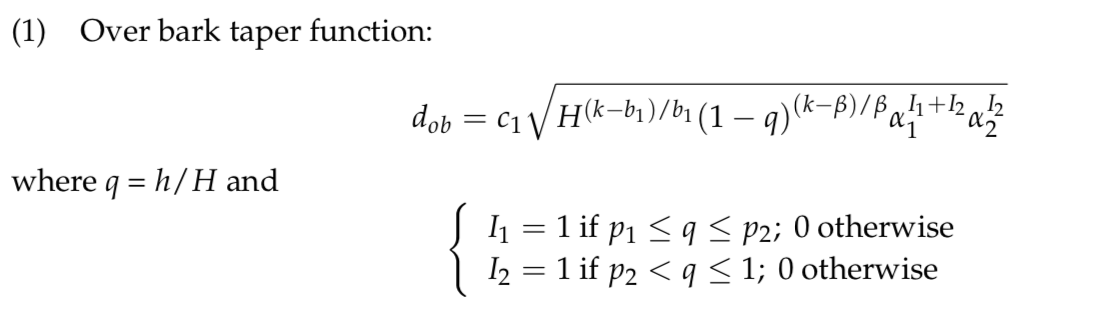
\includegraphics[width=0.8\textwidth]{Equations/2017Corral-RivasEtAlOb.png} \\ \hline
Equations & 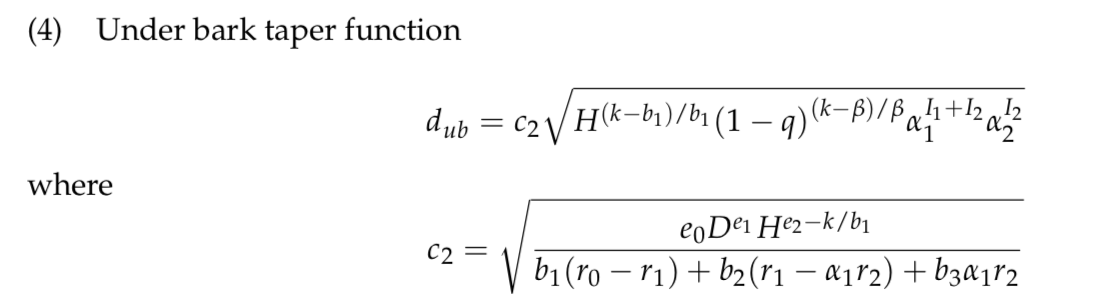
\includegraphics[width=0.8\textwidth]{Equations/2017Corral-RivasEtAlUb.png} \\ \hline
\end{tabular}

\captionof{table}{
Article ID 5 : _(Sun, Liang, Liang, et al., 2016)_
**Deriving {Merchantable} {Volume} in {Poplar} through a {Localized} {Tapering} {Function} from {Non}-{Destructive} {Terrestrial} {Laser} {Scanning}**
}
\begin{tabular}{p{0.2\textwidth} p{0.8\textwidth}}
\hline
Student & Matteo Piccolo \\ \hline
Title.student & Deriving Merchantable Volume in Poplar through a Localized Tapering Function from Non-Destructive Terrestrial Laser Scanning \\ \hline
Authors.student & Yuan Sun, Xinlian Liang, Ziyu Liang, Clive Welham and Weizheng Li \\ \hline
Year.student & 2016 \\ \hline
Species & Populus × canadensis Moench cv. \\ \hline
Base.URL & http://www.mdpi.com/1999-4907/7/4/87/htm \\ \hline
Paper.local.file & forests-07-00087.pdf \\ \hline
Equations & 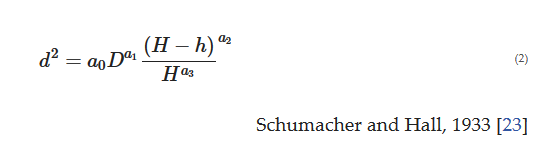
\includegraphics[width=0.8\textwidth]{Equations/2016Sunetal.png} \\ \hline
\end{tabular}

\captionof{table}{
Article ID 6 : _(Martins, Debastiani, Pelissari, et al., 2017)_
**Estimativa do {Afilamento} do {Fuste} de {Araucária} {Utilizando} {Técnicas} de {Inteligência} {Artificial}**
}

\textbackslash{}begin\{tabular\}\{p\{0.2\textwidth\}
p\{0.8\textwidth\}\} \hline Student \& NA \textbackslash{} \hline
Title.student \& Araucaria Stem Taper or Use of Artificial Intelligence
Techniques \textbackslash{} \hline Authors.student \& Ana Paula Marques
Martins, Aline Bernarda Debastiani, Allan Libanio Pelissari, Sebastião
do Amaral Machado, Carlos Roberto Sanquetta \textbackslash{} \hline
Year.student \& 2017 \textbackslash{} \hline Species \& Araucaria
angustifolia \textbackslash{} \hline Base.URL \&
\url{http://www.scielo.br/scielo.php?script=sci_arttext\&pid=S2179-80872017000100152}
\textbackslash{} \hline Paper.local.file \&
2179-8087-floram-24-e20160234.pdf \textbackslash{} \hline Equations \&
NA \textbackslash{} \hline \textbackslash{}end\{tabular\}

\captionof{table}{
Article ID 7 : _(Silva, Rodriguez, Caixeta Filho, et al., 2006)_
**Fitting a taper function to minimize the sum of absolute deviations**
}

\textbackslash{}begin\{tabular\}\{p\{0.2\textwidth\}
p\{0.8\textwidth\}\} \hline Student \& NA \textbackslash{} \hline
Title.student \& Fitting a taper function to minimize the sum of
absolute deviations \textbackslash{} \hline Authors.student \& Lana
Mirian Santos da Silva, Luiz Carlos Estraviz Rodriguez, José Vicente
Caixeta Filho; Simone Carolina Bauch \textbackslash{} \hline
Year.student \& 2006 \textbackslash{} \hline Species \& Eucalyptus
\textbackslash{} \hline Base.URL \&
\url{http://www.scielo.br/scielo.php?script=sci_arttext\&pid=S0103-90162006000500007}
\textbackslash{} \hline Paper.local.file \& 31406.pdf \textbackslash{}
\hline Equations \& NA \textbackslash{} \hline
\textbackslash{}end\{tabular\}

\captionof{table}{
Article ID 8 : _(Arnoni Costa, Guimarães Finger, Schneider, et al., 2016)_
**{FUNÇÃO} {DE} {AFILAMENTO} {E} {SORTIMENTOS} {DE} {MADEIRA} {PARA} {Araucaria} angustifolia**
}
\begin{tabular}{p{0.2\textwidth} p{0.8\textwidth}}
\hline
Student & NA \\ \hline
Title.student & Taper function and timber assortments for Araucaria angustifolia \\ \hline
Authors.student & Emanuel Arnoni Costa, César Augusto Guimarães Finger, Paulo Renato Schneider, André Felipe Hess \\ \hline
Year.student & 2016 \\ \hline
Species & Araucaria angustifolia \\ \hline
Base.URL & http://www.redalyc.org/articulo.oa?id=53446151016 \\ \hline
Paper.local.file & 53446151016.pdf \\ \hline
Equations & NA \\ \hline
\end{tabular}

\captionof{table}{
Article ID 9 : _(Souza, Chassot, Finger, et al., 2008)_
**Modelos de afilamento para o sortimento do fuste de {Pinus} taeda {L}**
}

\textbackslash{}begin\{tabular\}\{p\{0.2\textwidth\}
p\{0.8\textwidth\}\} \hline Student \& NA \textbackslash{} \hline
Title.student \& Taper function for assortment of Pinus taeda L. stem
\textbackslash{} \hline Authors.student \& Carlos Alberto Martinelli de
Souza, Tatiane Chassot, César Augusto Guimarães Finger, Paulo Renato
Schneider, Frederico Dimas Fleig \textbackslash{} \hline Year.student \&
2008 \textbackslash{} \hline Species \& Pinus taeda L \textbackslash{}
\hline Base.URL \&
\url{http://www.scielo.br/scielo.php?script=sci_arttext\&pid=S0103-84782008000900014}
\textbackslash{} \hline Paper.local.file \& a14v38n9.pdf
\textbackslash{} \hline Equations \& NA \textbackslash{} \hline
\textbackslash{}end\{tabular\}

\captionof{table}{
Article ID 10 : _(Arias-Rodil, Castedo-Dorado, Cámara-Obregón, et al., 2015)_
**Fitting and {Calibrating} a {Multilevel} {Mixed}-{Effects} {Stem} {Taper} {Model} for {Maritime} {Pine} in {NW} {Spain}**
}
\begin{tabular}{p{0.2\textwidth} p{0.8\textwidth}}
\hline
Student & NA \\ \hline
Title.student & Fitting and Calibrating a Multilevel Mixed-Effects Stem Taper Model for Maritime Pine in NW Spain \\ \hline
Authors.student & Manuel Arias-Rodil, Fernando Castedo-Dorado, Asunción Cámara-Obregón, Ulises Diéguez-Aranda \\ \hline
Year.student & 2015 \\ \hline
Species & Pinus pinaster Ait. \\ \hline
Base.URL & http://europepmc.org/backend/ptpmcrender.fcgi?accid=PMC4668033&blobtype=pdf \\ \hline
Paper.local.file & pone.0143521.pdf \\ \hline
Equations & NA \\ \hline
\end{tabular}

\captionof{table}{
Article ID 11 : _(Rodríguez, Lizarralde, and Bravo, 2015)_
**Comparison of stem taper equations for eight major tree species in the {Spanish} {Plateau}**
}
\begin{tabular}{p{0.2\textwidth} p{0.8\textwidth}}
\hline
Student & NA \\ \hline
Title.student & Comparison of stem taper equations for eight major tree species in the Spanish Plateau \\ \hline
Authors.student & Francisco Rodríguez1, Iñigo Lizarralde1 and Felipe Bravo \\ \hline
Year.student & 2015 \\ \hline
Species & Various \\ \hline
Base.URL & http://revistas.inia.es/index.php/fs/article/view/6229 \\ \hline
Paper.local.file & 6229-27194-1-PB.pdf \\ \hline
Equations & NA \\ \hline
\end{tabular}

\captionof{table}{
Article ID 12 : _(Návar, Rodríguez-Flores, and Domínguez-Calleros, 2013)_
**Taper functions and merchantable timber for temperate forests of northern {Mexico}**
}
\begin{tabular}{p{0.2\textwidth} p{0.8\textwidth}}
\hline
Student & NA \\ \hline
Title.student & Taper functions and merchantable timber for temperate forests of northern Mexico \\ \hline
Authors.student & J. Návar, F. de Jesús Rodríguez-Flores, P.A. Domínguez-Calleros \\ \hline
Year.student & 2013 \\ \hline
Species & P.pseudostrobus, P. hartwegii, P. cooperi, P. ayacahuite, Q. spp, P. durangensis, P. leiophylla, P. teocote, P. arizonica, Quercus spp \\ \hline
Base.URL & http://www.editurasilvica.ro/afr/56/1/navar.pdf \\ \hline
Paper.local.file & navar.pdf \\ \hline
Equations & NA \\ \hline
\end{tabular}

\captionof{table}{
Article ID 13 : _(Özçelik and Dirican, 2017)_
**Stem taper and volume models for natural cedar and {Taurus} fir mixed stands in {Bucak} {District}**
}
\begin{tabular}{p{0.2\textwidth} p{0.8\textwidth}}
\hline
Student & NA \\ \hline
Title.student & Individual taper models for natural cedar and Taurus fir mixed stands of Bucak Region, Turkey \\ \hline
Authors.student & Ramazan Özçelik, Osman Dirican \\ \hline
Year.student & 2017 \\ \hline
Species & Cedrus libani A. Rich., Abies cilicica Carr. \\ \hline
Base.URL & http://dergipark.gov.tr/download/article-file/330518 \\ \hline
Paper.local.file & 10.17099-jffiu.290845-330518.pdf \\ \hline
Equations & NA \\ \hline
\end{tabular}

\captionof{table}{
Article ID 14 : _(Machado, Urbano, and Conceição, 2005)_
**Comparação de métodos de estimativa de volume para {Pinus} oocarpa em diferentes idades e diferente iregimes de desbastes**
}
\begin{tabular}{p{0.2\textwidth} p{0.8\textwidth}}
\hline
Student & NA \\ \hline
Title.student & Comparação de Métodos de Estimativa de Volume para Pinus oocarpa em Diferentes Idades e Diferentes Regimes de Desbastes \\ \hline
Authors.student & Sebastião do Amaral Machado, Edilson Urbano, Marcio Barbosa da Conceição \\ \hline
Year.student & 2005 \\ \hline
Species & Pinus oocarpa \\ \hline
Base.URL & https://pfb.cnpf.embrapa.br/pfb/index.php/pfb/article/view/242/193 \\ \hline
Paper.local.file & 242-1027-1-PB.pdf \\ \hline
Equations & NA \\ \hline
\end{tabular}
\clearpage

\hypertarget{references}{%
\section{References}\label{references}}

Ã--zçelik, R. and O. Dirican (2017). ``Stem taper and volume models for
natural cedar and Taurus fir mixed stands in Bucak District''. In:
\emph{Ä°stanbul ÃÅ``niversitesi Orman Fakültesi Dergisi} 67.2,
pp.~1-1. ISSN: 0535-8418. DOI:
\href{https://doi.org/10.17099/jffiu.290845}{10.17099/jffiu.290845}.

Arias-Rodil, M, F. Castedo-Dorado, A. Cámara-Obregón, et al.
(2015). ``Fitting and Calibrating a Multilevel Mixed-Effects Stem Taper
Model for Maritime Pine in NW Spain''. En. In: \emph{PLOS ONE} 10.12.
Ed. by M. Reigosa, p.~e0143521. ISSN: 1932-6203. DOI:
\href{https://doi.org/10.1371/journal.pone.0143521}{10.1371/journal.pone.0143521}.

Arnoni Costa, E, C. A. Guimarães Finger, P. R. Schneider, et al.
(2016). ``FUNÇÃÆ'O DE AFILAMENTO E SORTIMENTOS DE MADEIRA PARA
Araucaria angustifolia''. Portugués. In: \emph{CiÃÆ'ªncia
Florestal} 26.2, pp.~523-533. ISSN: 0103-9954. (Visited on lug. 28,
2018).

Corral-Rivas, J, D. Vega-Nieva, R. Rodríguez-Soalleiro, et al.
(2017). ``Compatible System for Predicting Total and Merchantable Stem
Volume over and under Bark, Branch Volume and Whole-Tree Volume of Pine
Species''. En. In: \emph{Forests} 8.11, p.~417. ISSN: 1999-4907. DOI:
\href{https://doi.org/10.3390/f8110417}{10.3390/f8110417}.

Machado, S. d. A, E. Urbano and M. B. d. Conceição (2005).
``Comparação de métodos de estimativa de volume para Pinus
oocarpa em diferentes idades e diferente iregimes de desbastes''. In:
\emph{Pesquisa Florestal Brasileira} 2005.50 ( jan./jun.).

Martins, A. P. M, A. B. Debastiani, A. L. Pelissari, et al. (2017).
``Estimativa do Afilamento do Fuste de Araucária Utilizando
Técnicas de Inteligência Artificial''. In: \emph{Floresta e
Ambiente} 24.0. ISSN: 2179-8087. DOI:
\href{https://doi.org/10.1590/2179-8087.023416}{10.1590/2179-8087.023416}.

Návar, J, F. d. J. Rodríguez-Flores and P. A.
Domínguez-Calleros (2013). ``Taper functions and merchantable timber
for temperate forests of northern Mexico''. In: \emph{Annals of Forest
Research} 56.1. ISSN: 20652445.

Rodríguez, F, I. Lizarralde and F. Bravo (2015). ``Comparison of stem
taper equations for eight major tree species in the Spanish Plateau''.
In: \emph{Forest Systems} 24.3, p.~e034. ISSN: 2171-9845, 2171-5068.
DOI:
\href{https://doi.org/10.5424/fs/2015243-06229}{10.5424/fs/2015243-06229}.

Scolforo, H. F, J. P. McTague, M. R. Raimundo, et al. (2018).
``Comparison of taper functions applied to eucalypts of varying genetics
in Brazil: application and evaluation of the penalized mixed spline
approach''. En. In: \emph{Canadian Journal of Forest Research} 48.5,
pp.~568-580. ISSN: 0045-5067, 1208-6037. DOI:
\href{https://doi.org/10.1139/cjfr-2017-0366}{10.1139/cjfr-2017-0366}.

Silva, L. M. S. d, L. C. E. Rodriguez, J. V. Caixeta Filho, et al.
(2006). ``Fitting a taper function to minimize the sum of absolute
deviations''. In: \emph{Scientia Agricola} 63.5, pp.~460-470. ISSN:
0103-9016. DOI:
\href{https://doi.org/10.1590/S0103-90162006000500007}{10.1590/S0103-90162006000500007}.

Souza, C. A. M. d, T. Chassot, C. A. G. Finger, et al. (2008). ``Modelos
de afilamento para o sortimento do fuste de Pinus taeda L''. In:
\emph{Ciência Rural} 38.9, pp.~2506-2511. ISSN: 0103-8478. DOI:
\href{https://doi.org/10.1590/S0103-84782008000900014}{10.1590/S0103-84782008000900014}.

Sun, Y, X. Liang, Z. Liang, et al. (2016). ``Deriving Merchantable
Volume in Poplar through a Localized Tapering Function from
Non-Destructive Terrestrial Laser Scanning''. En. In: \emph{Forests}
7.12, p.~87. ISSN: 1999-4907. DOI:
\href{https://doi.org/10.3390/f7040087}{10.3390/f7040087}.

Tang, X, C. Pérez-Cruzado, L. Fehrmann, et al. (2016). ``Development
of a Compatible Taper Function and Stand-Level Merchantable Volume Model
for Chinese Fir Plantations''. En. In: \emph{PLOS ONE} 11.1. Ed. by R.
Wu, p.~e0147610. ISSN: 1932-6203. DOI:
\href{https://doi.org/10.1371/journal.pone.0147610}{10.1371/journal.pone.0147610}.

Warner, A. J, M. Jamroenprucksa and L. Puangchit (2016). ``Development
and evaluation of teak (Tectona grandis L.f.) taper equations in
northern Thailand''. En. In: \emph{Agriculture and Natural Resources}
50.5, pp.~362-367. ISSN: 2452316X. DOI:
\href{https://doi.org/10.1016/j.anres.2016.04.005}{10.1016/j.anres.2016.04.005}.


\end{document}
